\documentclass[utf8]{frontiersSCNS}

\usepackage{url,hyperref,lineno,microtype,subcaption,gensymb,booktabs}
\usepackage[onehalfspacing]{setspace}

\linenumbers

\def\keyFont{\fontsize{8}{11}\helveticabold }
\def\firstAuthorLast{Sample {et~al.}} %use et al only if is more than 1 author
\def\Authors{Robert W. Schlegel\,$^{1,*}$, Eric C. J. Oliver\,$^{2,3,4}$, Sarah Perkins-Kirkpatrick\,$^{5}$, Andries Kruger\,$^{6,7}$ and Albertus J. Smit\,$^{1}$}
% Affiliations should be keyed to the author's name with superscript numbers and be listed as follows: Laboratory, Institute, Department, Organization, City, State abbreviation (USA, Canada, Australia), and Country (without detailed address information such as city zip codes or street names).
% If one of the authors has a change of address, list the new address below the correspondence details using a superscript symbol and use the same symbol to indicate the author in the author list.
\def\Address{$^{1}$Department of Biodiversity and Conservation Biology, University of the Western Cape, Bellville, South Africa \\
$^{2}$Australian Research Council Centre of Excellence for Climate System Science, University of Tasmania, Hobart, Tasmania, Australia \\
$^{3}$Oceans \& Cryosphere, Institute for Marine and Antarctic Studies, University of Tasmania, Hobart, Tasmania, Australia \\
$^{4}$Department of Oceanography, Dalhousie University, Halifax, Nova Scotia, Canada \\
$^{5}$Climate Change Research Centre and ARC Centre of Excellence for Climate System Science, University of New South Wales, Sydney, Australia \\
$^{6}$Climate Service, South African Weather Service, Pretoria, South Africa \\
$^{7}$Department of Geography, Geoinformatics and Meteorology, University of Pretoria, Pretoria, South Africa}
% $^{x}$Laboratory X, Institute X, Department X, Organization X, City X , State XX (only USA, Canada and Australia), Country X  }
% The Corresponding Author should be marked with an asterisk
% Provide the exact contact address (this time including street name and city zip code) and email of the corresponding author
\def\corrAuthor{Department of Biodiversity and Conservation Biology, University of the Western Cape, Private Bag X17, Bellville 7535, South Africa}

\def\corrEmail{3503570@myuwc.ac.za}




\begin{document}
\onecolumn
\firstpage{1}

\title[Air-sea patterns during marine heatwaves]{Predominant atmospheric and oceanic patterns during coastal marine heatwaves} 

\author[\firstAuthorLast ]{\Authors} %This field will be automatically populated
\address{} %This field will be automatically populated
\correspondance{} %This field will be automatically populated

\extraAuth{}% If there are more than 1 corresponding author, comment this line and uncomment the next one.
%\extraAuth{corresponding Author2 \\ Laboratory X2, Institute X2, Department X2, Organization X2, Street X2, City X2 , State XX2 (only USA, Canada and Australia), Zip Code2, X2 Country X2, email2@uni2.edu}


\maketitle


\begin{abstract}
As the mean temperatures of the worlds oceans increase, it is predicted that marine heatwaves (MHWs) will occur more frequently and with increased severity however, it has been shown that variables other than increases in sea water temperature have been responsible for MHWs. To better understand these mechanisms driving MHWs we have utilised atmospheric (ERA-Interim) and oceanic (OISST, AVISO) data to examine the patterns around southern Africa during coastal ($\textless$400 m from the low water mark; measured \emph{in situ}) MHWs. Nonmetric multidimensional scaling (NMDS) was first used to determine that the atmospheric and oceanic states during MHW were different from daily climatological states. Self-organising maps (SOMs) were then used to cluster the MHW states into one of nine nodes to determine the predominant atmospheric and oceanic patterns present during these events. It was found that warm water forced onto the coast via anomalous ocean circulation was the predominant oceanic pattern during MHWs. Warm atmospheric temperatures over the subcontinent during onshore or alongshore winds were the most prominent atmospheric patterns. Roughly one third of the MHWs were clustered into a node with no clear patterns, which implied that they were not forced by a recurring atmospheric or oceanic state, but rather through the unpredictable chaos of the climate system. Because warm atmospheric and/or oceanic temperature anomalies were not the only pattern associated with MHWs, the current trend of a warming earth does not necessarily mean that MHWs will increase apace; however, aseasonal variability in wind and current patterns were shown to be central to the formation of coastal MHWs, meaning that where climate systems shift from historic records, increases in MHWs will likely occur.

\tiny
 \keyFont{ \section{Keywords:} marine heatwaves, code:R, coastal, atmosphere, ocean, \emph{in situ} data, reanalysis data, climate change} 
 %All article types: you may provide up to 8 keywords; at least 5 are mandatory.
\end{abstract}


\section{Introduction}
Extreme thermal events that occur in the ocean are classified here as `marine heatwaves' (MHWs) after \citet{Hobday2016}. These events may occur suddenly, anywhere in the world, and at any time of the year. Several large MHWs, and their ecological impacts, have already been well documented. The first being a 2003 MHW that negatively impacted as much as 80\% of the Gorgonian fan colonies in the Mediterranean \citep{Garrabou2009}. A 2011 MHW is now known to have caused a permanent roughly 100 km range contraction of the ecosystem forming-kelp species \emph{Ecklonia radiata} in favour of the tropicalisation of reef fishes and seaweed turfs along the southern coast of Western Australia \citep{Wernberg2016}. The damage caused by MHWs is not confined to demersal organisms or coastal ecosystems as demonstrated by a MHW in the North West Atlantic Ocean in 2012 that impacted multiple commercial fisheries \citep{Mills2013}. When extreme enough, such as `The Blob' that persisted in the North West Pacific Ocean from 2014 to 2016, a MHW may negatively impact even marine mammals and seabirds \citep{Cavole2016}. Besides increases in mortality due to thermal stress, MHWs may also lead to outbreaks of disease in commercially viable species, such as that which occurred during the 2015/16 Tasman Sea event \citep{Oliver2017}.

It is now possible to directly compare MHWs occurring anywhere on the globe during any time of year using a consistent definition developed by \citet{Hobday2016}, which was accompanied by the development of a statistical methodology for calculating these events. Whereas the metrics created for the measurement of MHWs allowed for the comparison of events, they did not directly reveal what may be causing them. Beyond common measurements, it is necessary to determine the predominant patterns that occur during MHWs in order to identify their physical drivers.

It has been assumed that coastal MHWs should either be caused by oceanic forcing, atmospheric forcing, or a combination of the two; however, the scale at which this forcing must occur in order to drive MHWs at the coast has yet to be determined. Recent research into the rates of co-occurrence between nearshore and offshore MHWs revealed that oceanic forcing from offshore (within the continental shelf) onto the nearshore ($\textless$400 m from the coast, \emph{i.e.} also referred to as local scale) was far less responsible for the formation of coastal MHWs than hypothesised \citep{Schlegel2017}. It is therefore necessary to consider broader meso-scale mechanisms that may be responsible for such events occurring at the local scale. For example, the 2011 Western Australia MHW \citep{Pearce2013} was caused by the aseasonal transport of warm water onto the coast due to a surge of the Leeuwin Current \citep{Feng2013, Benthuysen2014}. Oceanic forcing was also the main contributor of the anomalously warm water during the 2015/16 Tasman MHW when the southward flowing East Australian Current caused a convergence of heat there \citep{Oliver2017}. Conversely, \citet{Garrabou2009} were able to show that atmospheric forcing played a clear role in formation of the 2003 Mediterranean MHW. While more complex, \citet{Chen2015a} also showed that atmosphere-ocean heat flux could be attributed as the main forcing variable in the 2012 Atlantic MHW. The Blob however appears to have occurred due to the lack of advection of heat from surface waters into the atmosphere due to anomalously high sea level pressure \citep{Bond2015a}. Outside of these few examples for these well documented events there has been little progress in developing a global understanding of the forcing of MHWs, nor has a methodology been developed with the capacity to determine the probable drivers of multiple MHWs simultaneously.

In order to develop a methodology that could be used to investigate the potential atmospheric and/or oceanic forcing of multiple coastal MHWs within a single framework, an index of the mean synoptic atmospheric and oceanic states around southern Africa during the occurrence of these events was created, similar to \citet{Oliver2017atlas} for Eastern Tasmania. The daily climatology for the atmosphere and ocean around southern Africa were also calculated to determine if the MHW states differed from the expected daily values. After determining this distinction, the MHW states were clustered with the use of a self-organising map (SOM). The aim of the distinction and the clustering was to visualise meso-scale patterns in the atmosphere and/or ocean that occur during MHWs at coastal sites, and to be certain that these patterns were different from daily climatologies. We predicted that i) atmospheric and oceanic states during MHWs would differ from daily climatology states; ii) recurrent atmospheric and oceanic patterns would be revealed through clustering; and iii) the clustered patterns would aid in the development of a broader mechanistic understanding of the physical drivers of coastal MHWs.

\section{Material and Methods}
\subsection{Study region}
The \emph{ca}. 3,100 km long South African coastline provides a natural laboratory for investigations into the forcing of nearshore phenomena as it may be divided into three distinct sections, allowing for a range of meso-scale oceanic influences to be considered within the same research framework (figure \ref{figure1}); therefore, the extent of the study area was set at 10\degree E to 40\degree E and 25\degree S to 40\degree S. The range of temperatures experienced along all three coasts is large, and the gradient of increasing temperature from the border of Namibia (Site 1) to the border of Mozambique (Site 26) is nearly linear. The west coast of the country is distinct from the other two coasts as it is bordered by the Benguela Current, which forms an Eastern Boundary Upwelling System (EBUS) \citep{Hutchings2009} against the coast. Conversely, the east coast is dominated by a western boundary current, the Agulhas Current \citep{Luning1990}, a poleward flowing body of warm water. The south coast is also bordered by the Agulhas Current but differs from the east coast in that it experiences both shear-forced and wind-driven upwelling \citep{Lutjeharms2000a} in addition to having significantly more thermal variability than the other two coasts \citep{Schlegel2017}. The Agulhas and Benguela currents meet along the south coast of the subcontinent and rather than having a fixed border, the two range from the Cape Peninsula in the west, to the western portion of the Agulhas Bank in the east. The Agulhas Current retroflects upon coming into contact with the Benguela \citep{Hutchings2009} however, it will occasionally punch through into the South Atlantic. This event, known as Agulhas leakage, allows warm, saline eddies of Indian Ocean water to propagate into the Atlantic Ocean \citep{Beal2011}.

Atmospheric circulation over the study area is dominated by two quasi-stationary anticyclonic high pressure cells. The South Indian Ocean High (hereafter Indian high) is situated approximately on the eastern border of the study area and draws warm moist air towards the east coast, whereas the South Atlantic Ocean High (hereafter Atlantic high) is found to the west of the subcontinent and draws cool dry air onto the west coast \citep{vanHeerden1998}. To the south of the subcontinent, prevailing westerly winds blow south of these two high pressure cells \citep{vanHeerden1998}. From their annual mean mean wind patterns, these three atmospheric features can be discerned from figure \ref{figure1}. Summer heating may lead to the development of heat lows within the subcontinent, which tend to be absent during winter \citep{Tyson2000}, allowing for the Indian and Atlantic highs to link over land \citep{vanHeerden1998}. Additionally, the Indian and Atlantic highs, as well as the westerlies, move northwards during winter months, with the effect that the colder westerly winds influence the weather mostly along the southern parts of the sub-continent \citep{vanHeerden1998}. Atmospheric temperatures along the coasts are largely influenced by the cold Benguela on the west coast and warm Agulhas Current along the east and south coasts \citep{vanHeerden1998}.


% Figure 1


\subsection{Data}
\subsubsection{Atmospheric data}
To visualise a synoptic view of the atmospheric state around southern Africa during coastal MHWs (see sections `Marine heatwaves' and `Atmosphere-ocean state' below) we chose to use ERA-Interim to provide atmospheric temperatures (2 m above surface) and wind vectors (10 m above surface). ERA-Interim is a comprehensive global atmospheric model that assimilates a wide range of data to create short term forecasts for 60 vertical layers \citep{Dee2011}. These forecasts are then combined with the assimilated data again during each 12-hourly cycle \citep{Dee2011}. ERA-Interim is produced by the European Centre for Medium-Range Weather Forecasts (ECMWF, http://www.ecmwf.int/) and at the time of this writing the chosen variables were available for download from January 1st, 1979 to December 31st, 2016. The data used in this study were downloaded at a daily resolution on a 1/2\degree \: grid and within the latitude/longitude of the study region (figure \ref{figure1}).

\subsubsection{Oceanic data}
The \emph{in situ} coastal seawater temperature data used in this study were acquired from the \href{https://github.com/ajsmit/SACTN}{South African Coastal Temperature Network} (SACTN)\footnote{https://robert-schlegel.shinyapps.io/SACTN/}. These data are contributed by seven different organizations and are collected \emph{in situ} with a mixture of hand-held alcohol or mercury thermometers as well as digital underwater temperature recorders (UTRs). This data set currently consists of 135 daily time series, with a mean duration of 19.7 years, meaning that many the time series in this dataset are shorter than the 30 year minimum proscribed for the characterisation of MHWs (see `Marine heatwaves' section below) \citep{Hobday2016}. It is however deemed necessary to use these data when investigating extreme events in the nearshore ($\textless$400 m from the low tide mark) as satellite derived sea surface temperature (SST) values along the coast have been shown to display large biases \citep{Smit2013} or capture minimum and maximum temperatures poorly \citep{Smale2009, Castillo2010}. Whereas a 30+ year period is ideal for determining a climatology, ten years may serve as an acceptable bottom limit \citep{Schlegel2017}. Following on from the methodology laid out in \citet{Schlegel2017}, time series with more than 10\% missing data or shorter than 10 years in length were excluded from this research. Accounting for these 10 year length and 10\% missing data constraints, the total number of \emph{in situ} time series used in this study was reduced to 26, with a mean length of 22.3 years.

Research on oceanic reanalysis data around southern Africa have shown that none of the products currently available model the complex Agulhas Current well \citep{Cooper2014}. It was therefore decided to use remotely sensed data to determine the SST and surface currents in the study area.

SST within the study region was determined with the AVHRR-Only Optimum Interpolated Sea Surface Temperature (OISST) dataset produced by NOAA. NOAA OISST is a global 1/4\degree \: gridded daily SST product that assimilates both remotely sensed and \emph{in situ} sources of data to create a level-4 gap free product \citep{Banzon2016}. These data were averaged to a 1/2\degree \: grid to match the courser resolution of the ERA-Interim data. At the time of this writing these data were available for download from September 1st, 1981 to June 5th, 2017.

To determine ocean surface currents remotely on a daily global 1/4\degree \: grid, sea level anomaly (SLA) values are used to determine absolute geostrophic flows. The directional values of these flow vectors (U and V) were the values used in this study. These values were averaged to a 1/2\degree \: grid to maintain consistent spatial representation between the datasets. At the time of this writing these data were available from January 1st, 1993 to January 6th, 2017. These altimeter products were produced by Ssalto/Duacs and distributed by Aviso, with support from Cnes (http://www.aviso.altimetry.fr/duacs/). 

\subsection{Marine heatwaves (MHWs)}
We use the definition for a MHW given by \citet{Hobday2016} as ``a prolonged discrete anomalously warm water event that can be described by its duration, intensity, rate of evolution, and spatial extent'' as well as the methodology laid out in \citet{Hobday2016} for the analysis of MHWs in this research. The algorithm developed by \citet{Hobday2016} requires daily time series data and isolates MHWs by first establishing the daily climatologies for the given time series. This is accomplished by finding the range of temperatures for any given day of the year, and then pooling these daily values further with the use of an 11-day moving window, across all years. From this pool are calculated two statistics of interest: the first being the average climatology for each day, and the second being the 90th percentile threshold for each day. When the observed temperatures within a time series exceed this threshold for a number of days it may be classified as a discrete event. \citet{Perkins2013} concluded that the minimum duration for the analysis of atmospheric heatwaves was three days whereas \citet{Hobday2016} found that a minimum length of five days allowed for more uniform global results. It was also determined that any MHW that had `breaks' below the 90th percentile threshold lasting $\leq$2 days followed by subsequent days above the threshold were considered as one continuous event \citep{Hobday2016}. Previous work by \citet{Schlegel2017} showed that the inclusion of these short five day MHWs may lead to spurious connections between events found across different datasets. Therefore we have limited the inclusion of MHWs within this study to those with a duration in the top 10th percentile of all events that occurred within the range of complete years of data available for all of the datasets used in this study (1994--2016). Thus, from the 976 total MHWs detected in the \emph{in situ} dataset, only 86 were used here.

In order to calculate a MHW it is necessary to supply a climatology against which daily values may be compared. It is proscribed in \citet{Hobday2016} that this period be at least 30 years. Because 20 of the 26 time series used here are below this threshold we have opted to use the complete data period for each station as the climatological period. Using fewer than 30 years of data to determine a climatology prevents the accurate inclusion of any decadal scale variability \citep{Schlegel2016} however, by using at least 10 years of data we are able to establish a baseline climatology to calculate MHWs \citep{Schlegel2017}. By calculating MHWs against the daily climatologies in this way the amount they differ from their localities may be quantified and compared across time and space. Meaning that this allows researchers to examine events from different variability regimes (i.e. regions of the world, seasons) and compare them with a consistent set of MHW metrics. The definitions for the metrics that will be focused on in this paper may be found in table \ref{table1}.


% Table 1


The MHWs in the SACTN dataset were calculated via the R package `RmarineHeatWaves' \citep{Smit2017}. The original algorithm used in \citet{Hobday2016} is available for use via python \footnote{https://github.com/ecjoliver/marineHeatWaves}.

It is worth emphasising that MHWs as defined here exist against the daily climatologies of the time series in which they are found and not by exceeding an absolute threshold. Therefore, one may just as likely find a MHW during winter months as summer months. This is a valuable characteristic of this method of investigation because aseasonal warm winter waters may, for example, have deleterious effects on relatively thermophobic species \citep{Wernberg2011}, or aid the recruitment of invasive species \citep{Stachowicz2002}.

It must also be clarified that due to the irregular sampling effort in the SACTN dataset along the coastline of southern Africa, the spatial and temporal distributions of the 86 MHWs are not necessarily even. With some areas, specifically the south coast, having a much greater likelihood of MHWs that meet the selection criteria. This inequality in the data was not corrected for as the central purpose of this research was to determine the predominant atmospheric or oceanic states (see section `Atmosphere-ocean state' below) during the longest events in the dataset, regardless of where or when they occurred.

\subsection{Atmosphere-ocean states}
In order to visualise meso-scale patterns in the atmosphere and ocean around southern Africa during a coastal MHW it was necessary to first combine all of the daily values of these physical states for all days available across all of the datasets downloaded for this research (1994--2016). The oceanic states consisted of SST and surface currents while the atmospheric states were surface temperatures and surface winds. One mean atmosphere-ocean state was then created for each of the 86 MHWs in this study by taking the daily atmosphere-ocean states during each day during which the event occurred and averaging them together. For example, for a MHW that started on December 1st, 1999, and ended on March 7th, 2000, the 98 daily atmosphere-ocean states during that event were averaged to create a single atmosphere-ocean state that represented the overall pattern that was occurring during that one event. This example may be seen in the top row of panels in figure \ref{figure2}.

The calculation of the anomalies that would be used for all subsequent stages of this research required that a daily climatology be created for the atmospheric and oceanic states. These 366 daily atmosphere-ocean climatologies were calculated using the same algorithm used to determine the average daily climatologies for the \emph{in situ} time series, with the climatological period set from 1994 to 2016 as this was the widest period available across all of the gridded datasets. With the atmosphere-ocean climatology known for each calendar day of the year, it was then possible to subtract these daily climatologies from the daily atmosphere-ocean states during which a MHW was occurring before averaging each individual daily anomaly together to create one mean atmosphere-ocean anomaly state for each event. An example of the atmosphere-ocean anomaly states created in this way may be seen in the middle row of figure \ref{figure2}. The daily climatology anomaly states to be used for comparison against the MHW anomaly states (see section `Nonmetric multidimensional scaling (NMDS)' below) were created by subtracting the annual mean climatology state from all of the daily climatology states.


% Figure 2


\subsection{Nonmetric multidimensional scaling (NMDS)}
The goal of using Nonmetric multidimensional scaling (NMDS) to ordinate the MHW anomaly states (hereafter MHW states) and climatology anomaly states (hereafter climatology states) was not to perform a statistical analysis on the data, indeed no significance is tested, but rather to visualise how each state relates to every other state while simultaneously visualising the effects of the categorical variables on the data. The resultant bi-plot generated by NMDS allows one to visually inspect the relationship between MHW and climatology states, in order to determine if they share a common pattern, or are indeed dissimilar from one another. This is done by reducing the dimensionality of the atmosphere-ocean states down to a two-dimensional field that may be understood by humans. NMDS was chosen for this task as it is one of the most robust unconstrained ordination methods available \citep{Minchin1987}. The use of this technique may not be wide-spread in climate science, but we found that it was effective for reducing the dimensionality of the atmosphere-ocean states used here. The temperature, U and V variables were first scaled to a mean of zero across the common variables within the same pixels for all MHW and climatology states. These scaled values were then converted into a Euclidean distance matrix before being fed into the NMDS algorithm. An additional benefit of NMDS is that it allows for the strength of the influence of the categorical variables within the data to be displayed on the resultant bi-plot as vectors, where the length of each vector represents the amount of influence that categorical variable has, and the direction of the vector shows where on the two-dimensional plain the ordinated data points are being influenced towards. The categorical variables considered when ordinating the MHW and climatology states together were the season during which the day or event occurred/started, as well as if the value represented a MHW or a climatology.

It is important to note with NMDS that the two dimensions (i.e. x and y axes) along which each all data point are ordinated, do not represent any specific variables within the dataset. Instead these axes represent the algorithms best attempt at reducing the stress in the model from  constraining a multi-dimensional dataset into a two-dimensional visualisation \citep{Kruskal1964}. It therefore requires knowledge of the data being ordinated in order for the user to determine a best approximation for the general values most closely represented in the axes of ordination.

\subsection{Self-organising maps (SOMs)}
Several methods of clustering synoptic data have been employed in climate science. Of these K-means clustering is perhaps most often employed \citep[e.g.][]{Corte-Real1998, Burrough2001, Kumar2011}, with hierarchical cluster analysis (HCA) less so \citep[e.g.][]{Unal2003}. A newer technique, self-organizing maps (SOMs), has been gaining in popularity in climate studies \citep[e.g.][]{Cavazos2000, Hewitson2002, Morioka2010}. Here we have used a SOM to cluster the 86 MHW state anomalies.

The initialisation of a SOM is similar to more traditional clustering techniques \citep[e.g.][]{Jain2010} in that a given number of clusters (hereafter referred to as nodes) are declared by the user in order to instruct the SOM algorithm into how many nodes it should first randomly assign all of the data point \citep{Hewitson2002}. Each data point in this instance represents an atmosphere-ocean anomaly state during a MHW and consists of temperature, U and V anomalies, which reach a total 9774 variables each. Therefore, each SOM node is represented not by a single value, but by a 9774 value long reference vector. After all of the data points have been clustered into a node, the SOM then determines the most suitable reference vector for each node to represent the data therein \citep{Hewitson2002}. The data points are then reintroduced to the SOM and, based on Euclidean distance, each data point is then matched to the node of `best fit' \citep{Hewitson2002}. During this process the reference vectors for each node are modified as the SOM algorithm `learns' how best to refine them to fit the data points, while also learning how best to fit the nodes in relation to one another \citep{Hewitson2002}. This means that not only does the SOM algorithm update the goodness of fit for each node during each run of the data, it also better orients the nodes against one another and allows better clustering of higher densities of similar data points (MHW state anomalies) \citep{Hewitson2002}. This allows the user to see not only into which node a given data point (MHW state anomaly) best belongs in, but also what the relationship between the nodes may be and how prevalent certain MHW state anomalies are over others. Here we initially allowed the SOM algorithm to iterate this process 100 times. Analysis of the resultant SOM showed that little progress was made in the fitting of the data after 40 iterations, and so 100 iterations was deemed appropriate.

Because the SOM algorithm was not able to provide consistent results each time the analysis was run on these data, we opted out of using the default random initialization (RI) method for the SOM in favour of principal component initialization (PCI). PCI differs from RI in that it uses the two principal components of the dataset, as determined from a principal component analysis (PCA) to initialize the choice of node centres for the SOM \citep{Akinduko2016}. This allows the SOM model to recreate the same results when it is run on the same data.

The appropriate number of nodes to use in a cluster analysis is an important decision \citep{Gibson2016a}. This is because it is necessary to include enough nodes to view a broad range of synoptic states, but not so many that the differences between the nodes become meaningless. Calculating the within group sum of squares (WGSS) as more nodes were included showed that four could be satisfactory, but that at least six would be better. Ultimately we settled on nine nodes as this allowed for a wider variety of different synoptic atmosphere-ocean states to be separated out from one another, allowing for a better understanding of the dominant patterns that exist during coastal MHWs. As proposed in \citet{Johnson2013}, the nodes that are output by a SOM should be significantly different from one another to ensure that an excess of nodes has not been used. Running an analysis of similarity we found this to be true for the choice of nine nodes (\emph{p} = 0.001).

Once each MHW state anomaly was clustered into a node a further mean atmosphere-ocean state anomaly for each node was calculated by taking the average of all of the MHW state anomalies clustered within each node. It was these final mean atmosphere-ocean state anomalies that were taken as the nine predominant atmosphere-ocean patterns during coastal MHWs.

\section{Results}
\subsection{Ordination of states}
In order to determine any patterns in the differences between the MHW and climatology states, they were ordinated and plotted on a bi-plot together. Figure \ref{figure3} shows that the climatology states were clustered together in a central position while the MHW states were scattered along the top and bottom. Furthermore, the climatology states have been ordinated by season in a very contiguous manner with little seasonal pattern existing for the MHW states. The vectors in figure \ref{figure3} showing the influence of the categorical variable `Season' very clearly relate to the occurrence of the climatology states, and not to the season of occurrence for the MHW states. The vectors indicating the direction of influence for the categorical variable `State' (i.e. MHW state or climatology state) show that the climatology states tend to centre in the middle of the bi-plot, as we may see, but that the MHW states tend to be ordinated similarly towards states that occur during autumn months. It is important to remember that these results are in reality multi-dimensional, not two-dimensional, as shown here. This is why \ref{figure3} shows MHW states both above and below the climatology states even though the vector for MHW states appears similar to the autumn vector. That the climatology states vary along the x axis in order of their occurrence throughout the year indicates that the variance this represents is the change in mean atmospheric and oceanic temperature throughout the seasonal cycle. The variance along the y axis is less clear, though it most likely represents differences in currents and winds. This inference is supported by the positioning of the spring and autumn climatology states, which are more variable than winter and summer, further up and down the y axis. There is also a significant (\emph{p} = 0.002) relationship between the duration (days) of the MHW and its position along the y axis, with the shorter MHWs further from the centre of the bi-plot. The MHW states are distributed either above the summer/spring climatology states or below the autumn climatology states. Furthermore, very few MHW states were near climatology states of the same season (e.g. winter MHW states may generally be found above the summer climatologies or below the autumn climatologies). 


% Figure 3


\subsection{SOM nodes}
The nine predominant atmospheric and oceanic patterns around southern Africa during coastal MHWs may be seen in figure \ref{figure4}. Note that while the oceanic and atmospheric patterns for each node are shown in separate panels, all atmosphere and ocean variables were fed through the SOM together, meaning that the SOM had to consider both states when clustering them into nodes. The oceanic states appear to have been the most relevant criteria for clustering into the nodes in the top left corner, centred on Node 1, with nodes further away having less pronounced oceanic patterns. The nodes along the right edge, centred on Node 6, show that the primary influence for the clustering of MHW states there was the atmosphere. The further from Node 6 a node is placed, the less pronounced the atmospheric pattern becomes. The further from these two dominant points a node is, the less pronounced the patterns therein will become, as Node 7 shows.

MHWs that occurred during summer were the least common, only present in three nodes (figure \ref{figure5}), with winter \& spring events occurring more than twice as frequently (table \ref{table2}). Every node contained at least one spring event, and all but two nodes contained winter events. Three nodes lacked autumn events, but these were otherwise the most evenly distributed. Clustering of autumn, winter, and spring events that occurred over a range of years may be found in six of the nine nodes; however, the clustering of events that occurred within the same year is also consistent throughout the nodes. All but one of the nodes contained MHWs that were separated over large distances and by oceanographically dissimilar features. Additionally, only three of the 86 MHWs in this study occurred on the east coast and were clustered into nodes that had events from all three coasts.

Table \ref{table2} shows that the largest values for duration (\emph{D}), cumulative intensity (\emph{i\textsubscript{cum}}) and maximum intensity (\emph{i\textsubscript{max}}) were more than twice those of the smallest values. An individual description of each node may be found below, with a qualitative summary of the patterns given in table \ref{table3}. It is important to note that the wind and current anomalies shown in \ref{figure4} do not show the absolute strength/direction of travel, but rather how these values deviated from the daily climatologies for the days during the MHWs in those nodes. The annual mean wind and current vectors may be seen in figure \ref{figure1}.


% Figure 4


% Figure 5


% Table 2


% Table 3


\subsubsection{Node 1}
Node 1 showed the most striking oceanic pattern out of all of the nodes. The mean oceanic pattern from all of the MHW states clustered into this panel showed Agulhas Current leakage into the Atlantic as well as forcing onto the coastal region around the Cape Peninsula and potentially along the rest of the south coast. The SST anomalies along the coast, as well as in the open ocean were also the warmest of all the panels. The atmospheric temperature anomaly was mild relative to the other nodes but very strong north westerly wind anomalies were present to the west of the subcontinent and strong northerly wind anomalies to the east. The north-westerly wind anomalies continued to the south of the subcontinent and along the south coast up to the location of the occurrence of the most eastward MHW before encountering the Indian high and abating. Neither of the high pressure cells showed any real influence on the overland wind anomalies. Node 1 was unique in that all of the MHWs occurred during note only the same season (spring), but the same year (2004) as well. This also made it the node with highest concentration of spring events, as well as being one of only two nodes to have events that occurred on only one coast.

\subsubsection{Node 2}
Node 2 showed similar warm SST anomalies in the nearshore along the west and south coasts as Node 1, with open ocean anomalies being cooler. There appeared to be some onshore forcing and leakage of the Agulhas Current but it was not as strong as in Node 1. The atmospheric temperature and wind anomalies in this panel were slightly less than Node 1 as well. The wind anomaly patterns were shifted slightly more to the south west with the westerly wind anomalies along the bottom of the panel reaching further east. The anomalous offshore wind circulation did not appear to move onshore. The average duration of the events in this node were the shortest of all the nodes.

\subsubsection{Node 3}
Node 3 showed the most negative SST anomalies of all the nodes, with some warm SST anomalies still present along much of the three coasts. There were atypical surface currents occurring to the south west of the Cape Peninsula, similar to Nodes 1 and 2, but without clear onshore forcing. The overland atmospheric temperature anomalies were strong in this node with westerly wind anomalies pushing onshore along the west and south coasts from the south west and continuing overland. These onshore south-westerly anomalies were met on the eastern side of the subcontinent by neutral Indian high anomalies.

\subsubsection{Node 4}
Node 4 showed Agulhas leakage and onshore forcing with warm coastal SST anomalies along all three coasts, similar to Nodes 1 and 2. Warm open ocean SST and current anomalies were relatively even, with a large stretch of warmer SST anomalies and Agulhas retroflection along the bottom of the panel. Atmospheric temperature anomalies were relatively neutral, though slightly warmer over the subcontinent than the ocean. The wind anomalies were similar to Nodes 1 and 2, but with the largest westerly wind anomalies of all of the nodes. Of the 13 MHWs clustered into Node 4, 11 of them occurred during the same year, though over a span of several months. The events in this node had, on average, the second shortest durations, second lowest cumulative intensities, and the lowest maximum intensities. This node therefore serves as a good representations of atmospheric and oceanic states during the smaller events in this study.

\subsubsection{Node 5}
Node 5 showed some atypical currents to the south west of the Cape Peninsula, similar to most of the nodes. The SST anomalies during the events in this node were a mix of warm and cold, with very mild warm anomalies present along most of the coast. The atmospheric temperature anomalies, particularly overland, were strong during these events. Even though the wind anomalies were slight over the ocean during the events in this node, they were stronger overland where anomalous onshore wind movement occurred. This is also one of only two nodes that contain an event that occurred on the east coast. The average maximum intensity for the events in this node is very nearly the greatest.

\subsubsection{Node 6}
The surface current and SST anomalies in Node 6 were very similar to Node 5, with fewer warm SST anomalies along the coast. The atmospheric temperature anomalies overland during these events were in excess of 7\degree C with strong south-easterly wind anomalies pushing not only onshore, but along the entire study area as well. The events clustered into this node had the greatest atmospheric temperature anomalies of all the nodes. Node 6 also shows a strong affinity for events from only one season, with 13 of the 16 MHW therein having occurred during winter, but were spread out from 1993 to 2014. This large concentration of winter events means that nearly half of all winter events were clustered into Node 6. The events in Node 4 battle those in Node 6 for the position of shortest and weakest, making this node another good example of the atmospheric and oceanic patterns during the smaller events used in this study. This node also has the greatest number of events clustered into it.

\subsubsection{Node 7}
Node 7 showed some atypical currents to the south west of the subcontinent but little in the way of onshore forcing or warm SST anomalies. The Southern Ocean appeared to be pushing up into the study area during these events as seen by the cold anomaly in the bottom middle of the panel. The atmospheric temperatures showed a very slight negative anomaly over much of the study area with very weak westerlies winds anomalies along the southern portion of the study area. That this node does not show any real patterns is not surprising given its position in relation to the nodes with stronger patterns. This node has the second greatest number of events clustered into it and contains half of all of the summer events in this study. These events also have the second longest average duration, the greatest average cumulative intensity, and the third greatest average maximum intensity. Because the node with the overall largest events only has two events clustered into it, Node 7 serves as the best representation of the atmospheric and oceanic patterns during very large events. 

\subsubsection{Node 8}
Node 8 showed warm SST anomalies for all but the offshore portion of the Atlantic Ocean. There was some atypical vorticity along the south of the study area, but this was moving away from the coast and there appeared to be little leakage of the Agulhas Current. The atmospheric temperature anomalies during these events were small with strong easterly wind anomalies moving across the entire study area. These wind anomalies wrapped around the subcontinent, and were not found overland. This node contained two of the three events that occurred on the east coast, and the third highest total of events clustered into a single node.

\subsubsection{Node 9}
The final node showed cold SST anomalies along much of the south and west coasts, with some warm anomalies further south of the subcontinent and atypical vorticity to the south east that did not appear to be reaching the coast. Easterly wind anomalies were found along the bottom of the study area with warm atmospheric temperature anomalies throughout. There are some slight onshore wind anomalies along the entire coastline. This is the only Node that contains events from only one location (site 1; figure \ref{figure1}). The two events clustered into this node have between them the greatest duration and maximum intensity, with the second greatest cumulative intensity. This makes the events in this node the overall largest however, the low number of events clustered here prevent this node from being a good indicator of a common atmospheric or oceanic pattern.

\section{Discussion}
\subsection{MHW states}
The ordination of the MHW and climatology states has shown that they do differ in discernible ways. The clustering of the climatology states in the centre of figure \ref{figure3} serves as a reference for better understanding the positioning of the MHW states. Because the proximity of points in an ordinated space shows their (dis)similarity to one another, the closer to the climatology states a MHW state may be found, the more it resembles it. This may seem contradictory at first given that all of the MHW states are ordinated most closely to climatology states that occurred during a different season. This means however that the states during all of th MHWs were aseasonal, and were more similar to climatology states during a different season of the year than the one in which they occurred. That none of the MHW states were ordinated near a winter climatology state is not surprising, as one would assume that MHWs should occur during warmer atmospheric or oceanic states. Following on this logic, a further assumption would be that the MHW states should most closely resemble the warmest time of year, summer. That the MHW states are instead ordinated more closely with autumn and spring climatology states means that high atmospheric or oceanic temperatures may be necessary for a MHW to occur, but are not the only driving force. During summer and winter months in southern Africa the Atlantic and Indian highs tend to stay in place latitudinally \citep{vanHeerden1998}. It is during autumn and spring that, not always in a predictable manner, the synoptic atmospheric features around the subcontinent migrate north or south \citep{vanHeerden1998}. As these systems shift they apparently create wind and/or current states that appear to be most similar to those that occurred during the coastal MHWs in this study. That high atmospheric and/or oceanic temperatures are not the only factor in the ordination of these MHW states is good as, under a warming global climate \citep{Pachauri2014}, this would likely mean an increase in MHWs. Instead we have found that it is aseasonality that is most consistently associated with MHW states. Therefore we may conclude that areas that experience increasingly divergent winds or currents from historical standards, without increasing temperatures, may also see an increase in MHWs.

Lastly, we have shown that in this ordinated space, the duration of the MHW around which each MHW state has been created, had a significant relationship with the proximity of the MHW state to climatology states. This is because the longer the event is, the more days of atmospheric and oceanic data are averaged together, creating a smoother and smoother state, that will more closely resemble one of the climatology states. This is a potential, though unavoidable weakness in the methodology.

\subsection{Agulhas leakage}
The most notable oceanic pattern from the clustering of these events into nodes with the use of a SOM has been Agulhas leakage. This phenomenon is when warm Indian Ocean water finds its way into the colder Atlantic Ocean \citep{Beal2011}. These warm eddies then typically spin up along the west coast. This transport of a large body of atypically warm water along a large stretch of coastline is a similar finding to the cause of the Western Australia MHW in 2011 where an unusual surge of the Leeuwin Current forced a large body of anomalously warm water onto the coast \citep{Feng2013, Benthuysen2014}. This onshore forcing of water is most apparent in Node 1 (figure \ref{figure4}) however, Nodes 2 and 4 show a similar though less pronounced oceanic pattern, meaning that roughly one third of the events in this study occurred during Agulhas leakage. These three Agulhas leakage-dominated nodes also share the same anomalously warm atmospheric temperatures and north westerly to westerly wind anomaly patterns, to varying degrees. Therefore we may conclude that the predominant oceanic pattern during coastal MHWs is warm coastal SST anomalies occurring during Agulhas leakage while strong north-westerly wind anomalies exists along the west coast of the subcontinent, weak south-easterly wind anomalies along the east coast, and westerly wind anomalies that may be drawing aseasonally close to the south coast of the subcontinent. One of the primary causes of Agulhas leakage is when a weak Indian high does not provide enough of the positive wind stress curl the current needs to have enough inertia to retroflect upon meeting the Benguela current \citep{Beal2011}. The second feature that allows Agulhas leakage is when the latitude zero wind stress curl caused by the westerly wind belt has shifted further south of the subcontinent \citep{Beal2011}. We see in the Agulhas leakage panels that wind anomalies around the Indian high are much weaker than the Atlantic high. This could potentially be allowing for a loss in inertia of the Agulhas Current and an increased risk of leakage however, the westerlies appear to be shifted further north, which should inhibit leakage. These two diametric forces contributing to the atmospheric and oceanic states during the Agulhas leakage may be what is causing the Agulhas to move so close to the shore, leading to the large SST anomalies seen there. Research has shown that 

Node 8 also shows some onshore forcing of the Agulhas Current, but with no large leakage into the Atlantic Ocean. Strong nearshore SST anomalies exist, but no ensuant leakage into the Atlantic due to the strong easterly wind anomalies over the Atlantic Ocean during the events in Node 8 that likely increased the inertia of the Agulhas Current enough that it retroflected upon meeting the Benguela current, while still forcing warm water onto the coast. Node 8 is also one of only two nodes that contain events from all three coasts, meaning that a strong Agulhas pushing onto the coast is a common pattern during MHW along the coastline of the entire study area.

Taken together with the events that occurred during Agulhas leakage, over half of the MHWs in this study occurred during some sort of anomalous Agulhas behaviour coupled with warm nearshore SST anomalies. This is strong support for the relationship between the Agulhas Current and coastal MHWs. \citet{Beal2011} state, while difficult to say with certainty, Agulhas leakage is likely to increase under the continued regime of global anthropogenic warming. \citet{Biastoch2009} also found that Agulhas leakage is likely to increase, though due to the poleward shift of westerly winds. It is therefore likely that large MHWs like those seen in Nodes 1, 2, 4 and 8 are will become more frequent.

\subsection{Onshore winds}
With the exception of Nodes 7 and 8, all of the atmospheric states during coastal MHWs showed warm atmospheric temperature anomalies that were greater over the subcontinent than the ocean. The wind anomaly patterns during coastal MHWs were either strong north-westerly anomalies over the Atlantic with weak south-easterly anomalies over the Indian Ocean, or the inverse, but always showed some wind anomalies moving onshore. Furthermore, the nodes with the greatest overland atmospheric temperature anomalies (3, 5, 6, and 9) had comparable amounts of cold and warm SST anomalies as well as onshore wind anomalies. This implies that the MHWs in these nodes were forced by the onshore wind anomalies occurring during warm atmospheric anomalies and not by oceanic conditions. From this the conclusion may be drawn that MHWs forced by atmospheric variability will almost certainly occur during warm atmospheric anomalies with onshore wind anomalies. This pairing of atmospheric anomalies may cause MHWs in one of three ways. The first would be through direct atmospheric heating of the shallow nearshore water, as occurred over the Mediterranean in 2003 \citep{Garrabou2009}. The second could be that the anomalous onshore wind movement could have prevented seasonally regular wind forced upwelling from occurring, which would have then caused the coastal water at the location of the event to appear aseasonally warm. Lastly it is possible that the aseasonal wind anomalies could have acted upon the Agulhas Current, causing it to weaken and thereby broaden out over the Agulhas Bank and seeping warm water onto the cost. Taken together the events in these nodes (3, 5, 6, and 9) account for roughly one third of the events in this study.

\subsection{Other patterns}
The lack of a strong atmospheric or oceanic pattern in Node 7 implies that the 15 events that were clustered there do not share any common pattern. Meaning that there may still be many MHWs that occur not because of any recurrent or predominant atmospheric or oceanic pattern. This is an important finding as it shows that even though clear patterns in atmosphere and ocean may exist during most MHWs, these events may still occur during entirely novel conditions. A different interpretation of the lack of an apparent pattern in Node 7 is that because the events clustered into that event were the longest, on average, of all of the events in this study, creating a mean atmospheric and oceanic state for the entire duration of each event was impractical. That enough variation in atmosphere and ocean would have occurred over the lifespan of the event so as to `smooth out' any apparent signal. If this is so, it does not serve to address what may have caused such a large event. Upon closer inspection, the \href{https://github.com/schrob040/AHW/tree/master/graph/synoptic}{atlas figures} for each event in Node 7 show that there are indeed patterns in the atmospheric and oceanic anomalies during these events, and that they do differ from the patterns in the other nodes.

The most seasonally predictable MHWs, those occurring during winter months and clustered into Node 6, where also the shortest and weakest. As these events were clearly a product of thermal heating, one could be lead to assume that atmospheric forcing of MHWs causes less dramatic events than those forced by the ocean. This assumption would be an incorrect as the MHWs clustered in Node 5, which also contain a clear atmospheric signal, have a greater cumulative intensity than most of the Agulhas leakage-dominated nodes. The largest events, those in Node 7, contain such disparate atmospheric and oceanic states that the mean atmospheric and oceanic patterns appear to be almost blank. These factors prevents a conclusion to be drawn on whether the atmosphere or ocean may cause the largest MHWs.

A final note on the patterns visible in figure \ref{figure4}. The south west corners of the oceanic states in Nodes 2, 3, 5, 6, 7, and 9, show an almost identical anticyclonic (clockwise) anomaly on the exact same pixels. Upon more minute investigation it was determined that this anticyclone, likely an Agulhas ring \citep{Hutchings2009}, occurred between roughly 12.5\degree E to 14.5\degree E and 35.5\degree S to 37.5\degree S. This eddy occurred during exactly two thirds of all of the events in this study, making it the most common atmospheric or oceanic pattern found.


\section{Conclusions}
This research has shown that not only are the atmosphere and ocean states during coastal MHWs not closely related to the daily climatology states seen throughout the year, that what similarities do exist between MHW and climatology states are completely aseasonal. This means that the patterns that occur during MHW states are always more closely related to a different season than the one in which they occurred. Furthermore, the fewest MHWs occurred during summer months than any other season. These two facts taken together support the argument that MHWs are not simply a symptom of solar heating during the warm months of the year, but that aseasonal winds and/or currents are also necessary for a coastal MHW to occur. It is also possible that MHWs are recorded less frequently during summer months because coastal waters will be warmer, and incursions of offshore water, or atmospheric heating will not cause a large enough difference in the expected daily temperatures to be flagged as a MHW.

The predominant oceanic pattern that emerged from the SOM clustering of the MHW states was the abnormal advection of warm water onto the coast in association with Agulhas Current leakage. The predominant atmospheric state was anomalously warm air centred over the subcontinent coinciding with strong onshore winds. The node containing the most long, cumulatively intense events lacked any patterns. Meaning that the majority of the MHWs in this study that had the potential to cause the most harm to nearshore ecosystems, there does not appear to be a consistent or recurrent atmospheric or oceanic pattern. Rather, most of the largest events occurred during a novel atmospheric and/or oceanic state that was not repeated often enough to receive their own node. A third smaller scale pattern was found to occur more frequently than both the predominant atmospheric and oceanic patterns detailed here. This was a sub-meso-scale anticyclonic eddy, roughly two degrees wide, and centred at 13.5\degree E and 36.5\degree S. We did not investigate the ocean dynamics implied by the presence of this eddy as that was beyond the scope of this study.

The methodology utilised here has shown that it is possible to discern predominant atmospheric and oceanic patterns that occur during MHWs; however, one must have knowledge of the meso-scale oceanic and atmospheric properties of the study area in order to correctly interrogate the results. Even with this knowledge, many of the largest MHWs did not show any relationship to these potential meso-scale forces. One must therefore not assume that such broad patterns in either the atmosphere or ocean must be forcing any single MHW observed in nearshore environments.

In order to determine potential patterns that may or may not exist during MHWs, this study utilised atmospheric and oceanic surface temperatures and velocity vectors. This was done because of the few large MHWs whose causes have been discerned \citep[e.g.][]{Garrabou2009, Feng2013, Pearce2013, Benthuysen2014, Chen2015a, Oliver2017}, most were related to these variables. Having shown that temperature and surface vorticity patterns do exist during coastal MHWs, a follow up to this study should analyse surface pressure, which was the main driver of the The Blob \citep{Bond2015a}, as well as eddy kinetic energy (EKE), which was a primary driver of the 2015/16 Tasman Sea MHW \citep{Oliver2017}.


\section*{Conflict of Interest Statement}
%All financial, commercial or other relationships that might be perceived by the academic community as representing a potential conflict of interest must be disclosed. If no such relationship exists, authors will be asked to confirm the following statement: 
The authors declare that the research was conducted in the absence of any commercial or financial relationships that could be construed as a potential conflict of interest.


\section*{Author Contributions}
The central concept of developing a `Marine Heatwave Atlas' was first developed and implemented for Tasmania by EO with input from SP. RS then adapted this concept for use in South Africa. The idea to cluster recurrent atmospheric and oceanic states during marine heatwaves was also first implemented by EO with input from SP. The SACTN and ERA-Interim data were acquired by RS. The Aviso and OISST data were acquired by AS. All analyses, figures, and tables were performed or created by RS, with many of them adapted from earlier work performed by EO. All results were initially interpreted and drafted by RS, with EO, SP, AK, and AS providing two rounds of critical revisions on the developing manuscript. EO and AS provided additional insights into the oceanography of southern Africa while SP and AK provided additional insights into the meteorology. All authors give approval for the submission of this manuscript for review and agree to be accountable for all aspects of the work.


\section*{Funding}
This research was supported by NRF Grant number CPRR14072378735 and ARC grant number DE140100952.


\section*{Acknowledgements}
We would like to thank DAFF, DEA, EKZNW, KZNSB, SAWS and SAEON for contributing all of the raw data used in this study. Without it, this article and the South African Coastal Temperature Network (SACTN) would not be possible. This paper makes a contribution to the objectives of the Australian Research Council Centre of Excellence for Climate System Science (ARCCSS). The data and analyses used in this paper may be downloaded at https://github.com/schrob040/MHW. The metadata for each SACTN time series used in this study may be downloaded at https://github.com/schrob040/AHW/blob/master/setupParams/SACTN\_site\_list.csv.


\bibliographystyle{frontiersinSCNS_ENG_HUMS}
\bibliography{AHW}


\section*{Figure captions}

\begin{figure}[]
\begin{center}
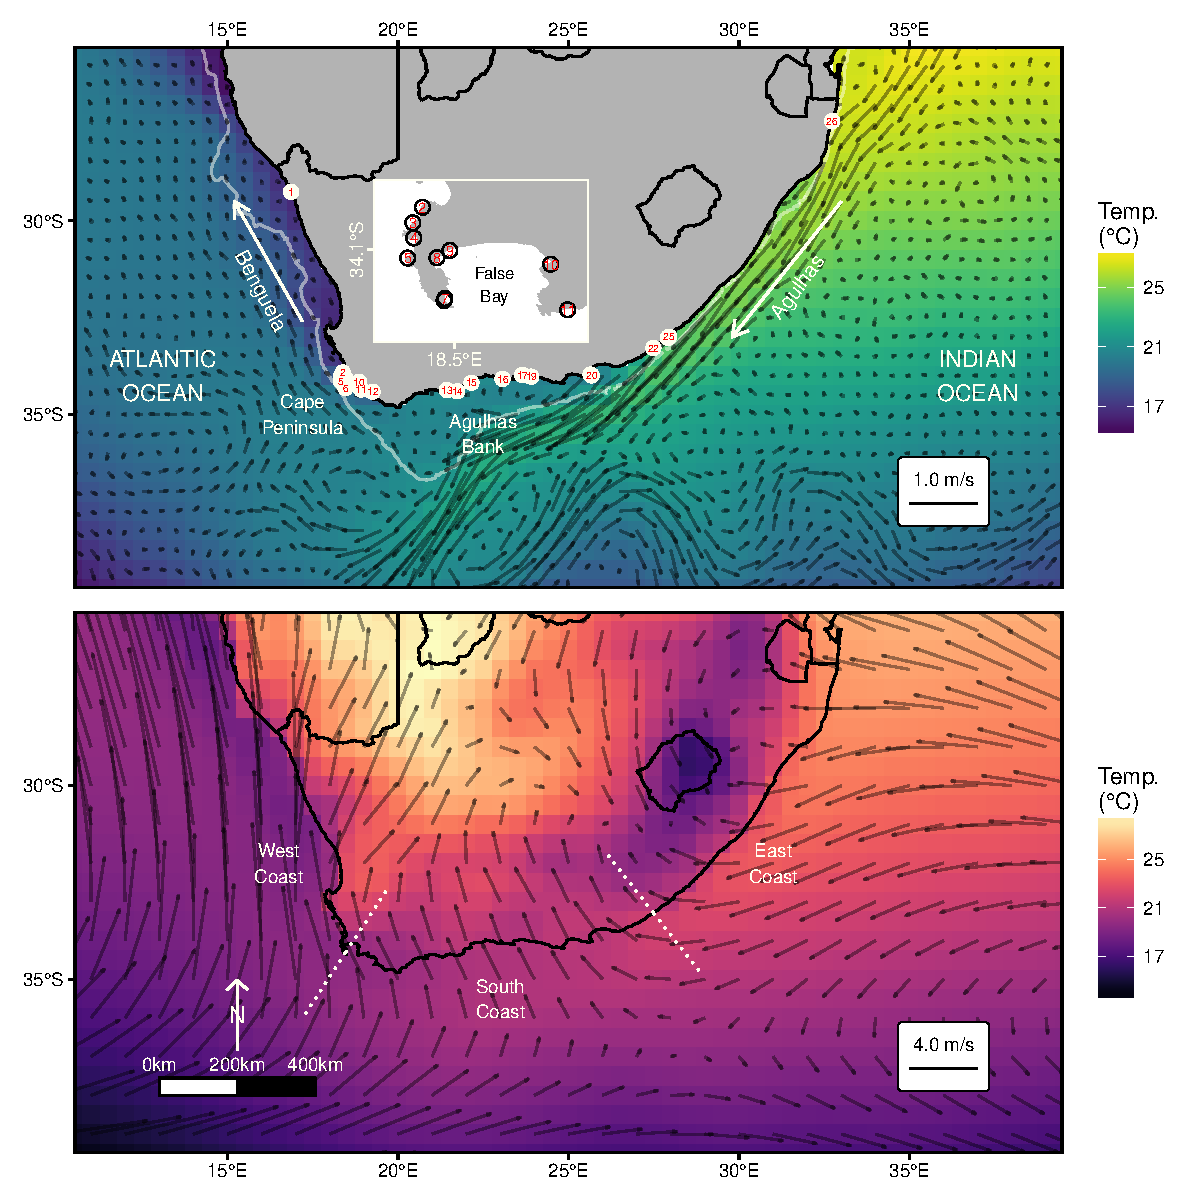
\includegraphics[width=1.0\textwidth]{figure_1.pdf}
\end{center}
\caption{Map of the study area where the top panel shows the mean annual sea surface temperature (SST) and surface currents from 1993 to 2016, as well as the locations referred to in the text. The sites of \emph{in situ} collection are shown with red numerals over white circles. An inset map of the Cape Peninsula/False Bay area is shown where site labels are obscured due to overplotting. The bottom panel shows the mean surface atmospheric temperature and winds, and highlights the three coastal sections found within the study area as well as the three predominant wind patterns. Note that the temperature and vector scales differ between the two panels. The white vector arrows showing the predominant ocean and atmosphere circulation patterns are approximations and not exact values.}
\label{figure1}
\end{figure}

\begin{figure}[]
\begin{center}
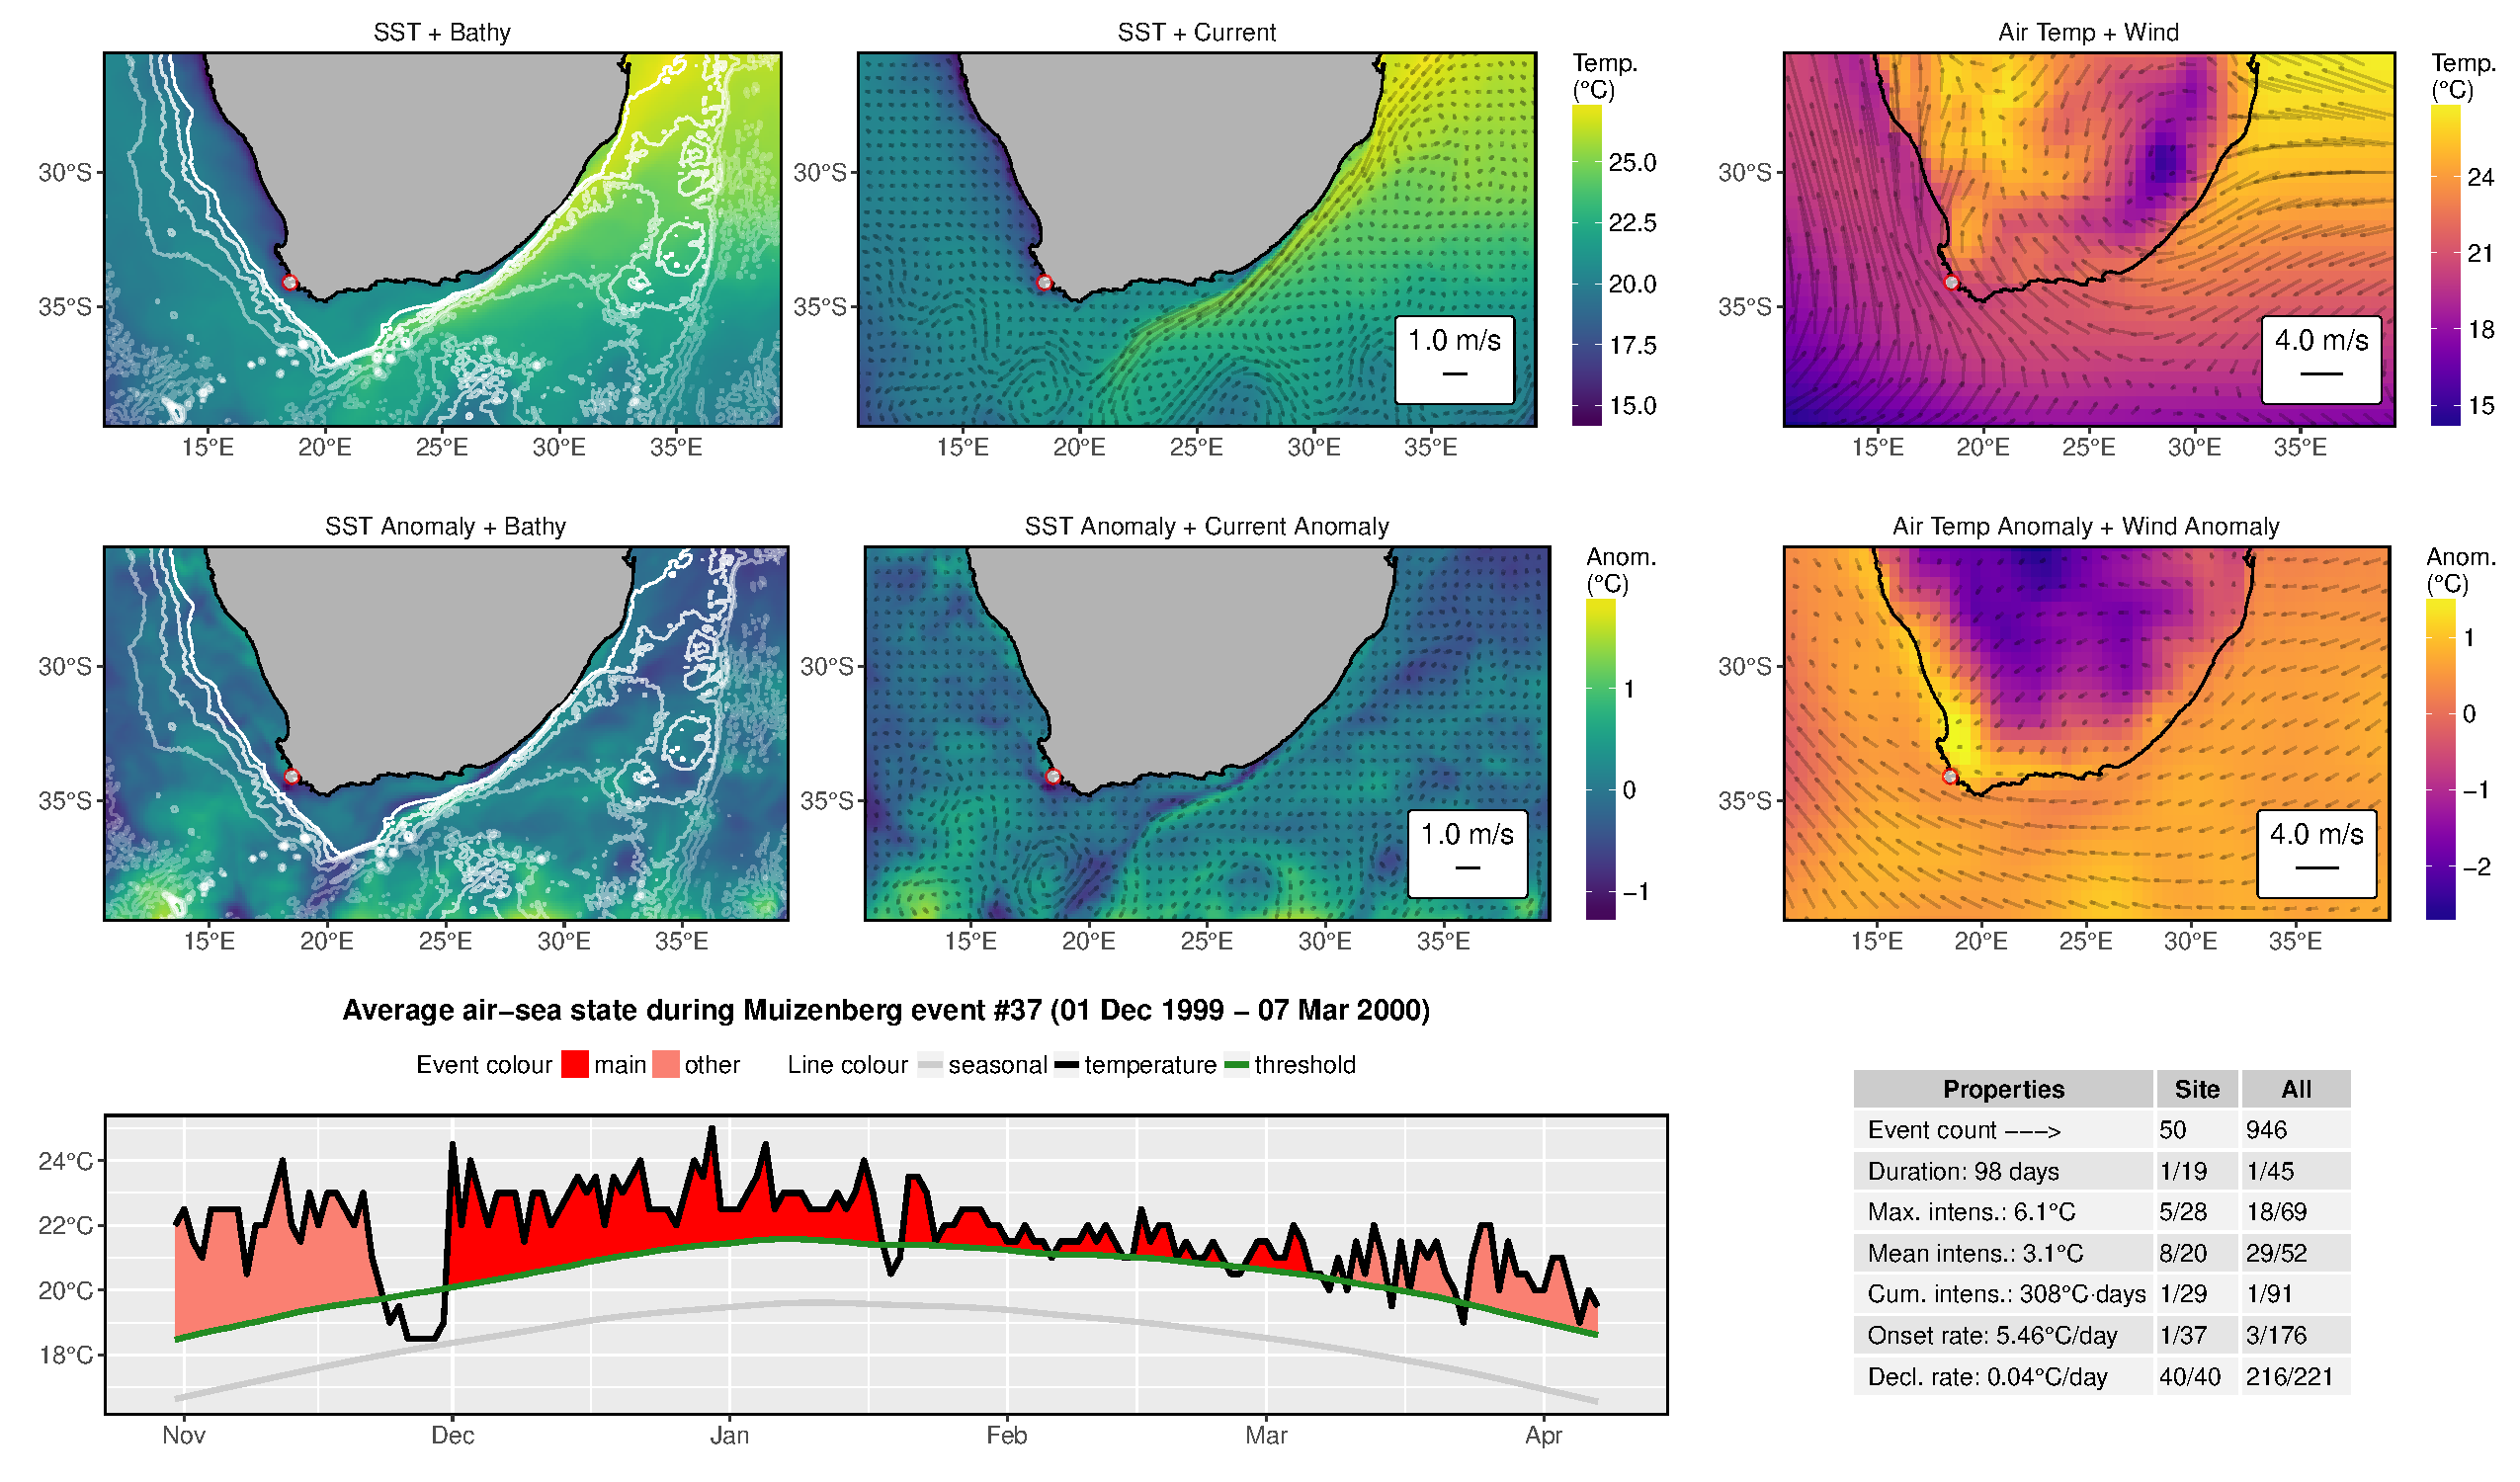
\includegraphics[width=1.0\textwidth]{figure_2.pdf}
\end{center}
\caption{An atlas figure for a single coastal marine heatwave (MHW). The location of collection for the \emph{in situ} coastal seawater temperature time series is shown in each of the top six panels as a white dot with a red border. The top row of panels shows the mean synoptic atmospheric and oceanic states during the MHW, created by averaging all daily synoptic atmosphere-ocean states during the event. The middle row shows anomalies for the mean atmospheric and oceanic states during the event. The left hand panel in the bottom row shows the period of the time series in which the MHW occurred. The table in the bottom right corner shows the values for the relevant metrics of the event as explained in table \ref{table1} as well as its ranking against other events at the same site and the entire study area. Similar figures for each of the 86 MHWs used in this study are available \href{https://github.com/schrob040/AHW/tree/master/graph/synoptic}{here}.}
\label{figure2}
\end{figure}

\begin{figure}[]
\begin{center}
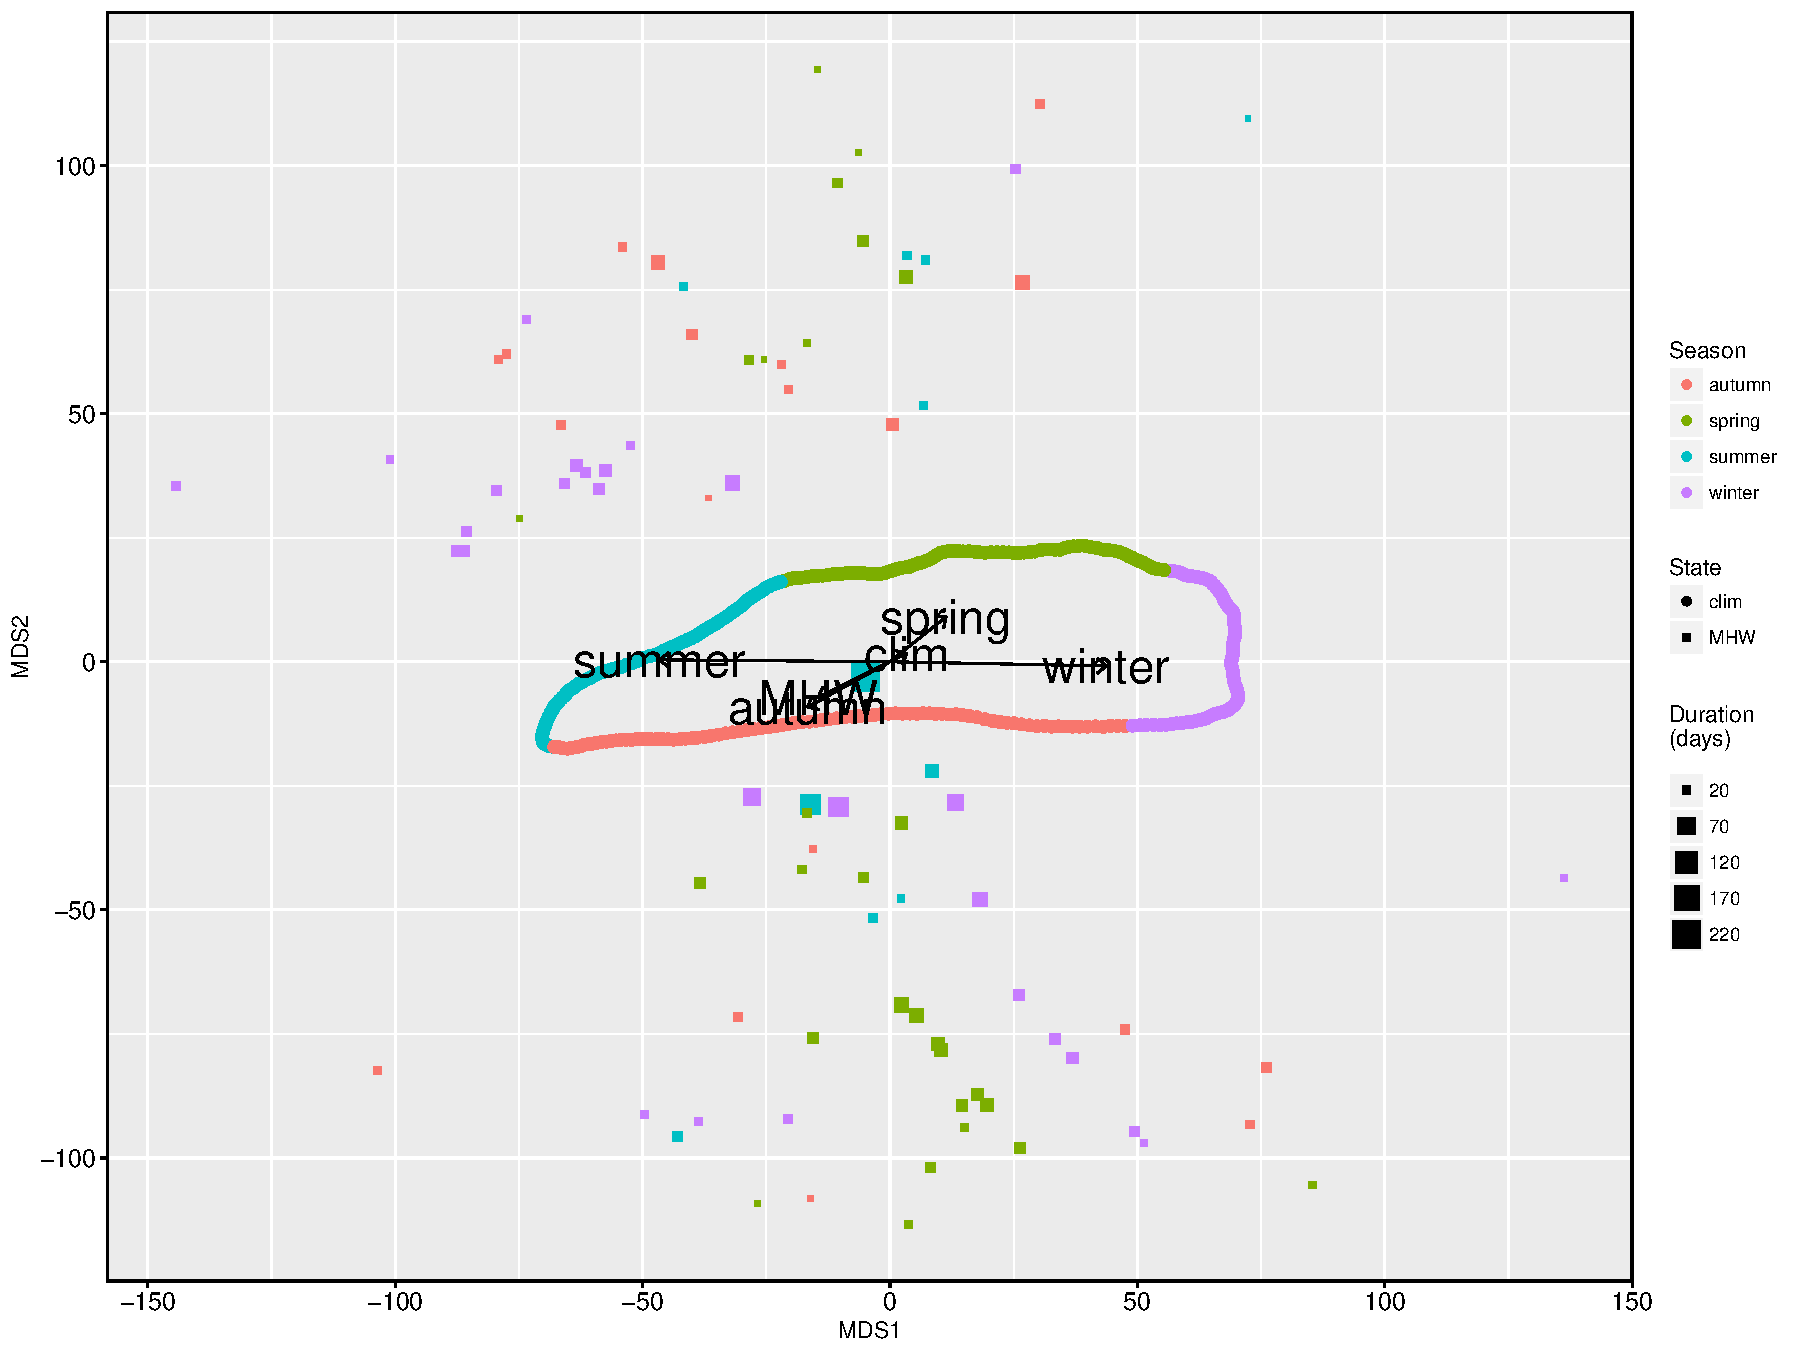
\includegraphics[width=1.0\textwidth]{figure_3.pdf}
\end{center}
\caption{Bi-plot showing the ordination of climatology (clim) states (circles) and marine heatwave (MHW) states (squares). The season of the year during which the state occurred/started is shown in colour. The influence of these two categorical variables, type of atmosphere-ocean state and season of occurrence, on the placement of each state in a two-dimensional space are shown as black labelled vectors. Note that the clim states (circles) are plotted so tightly together that they do not appear as individual points. The duration of the MHW states, but not the clim states, are indicated by the size of the square points.}
\label{figure3}
\end{figure}

\begin{figure}[]
\begin{center}
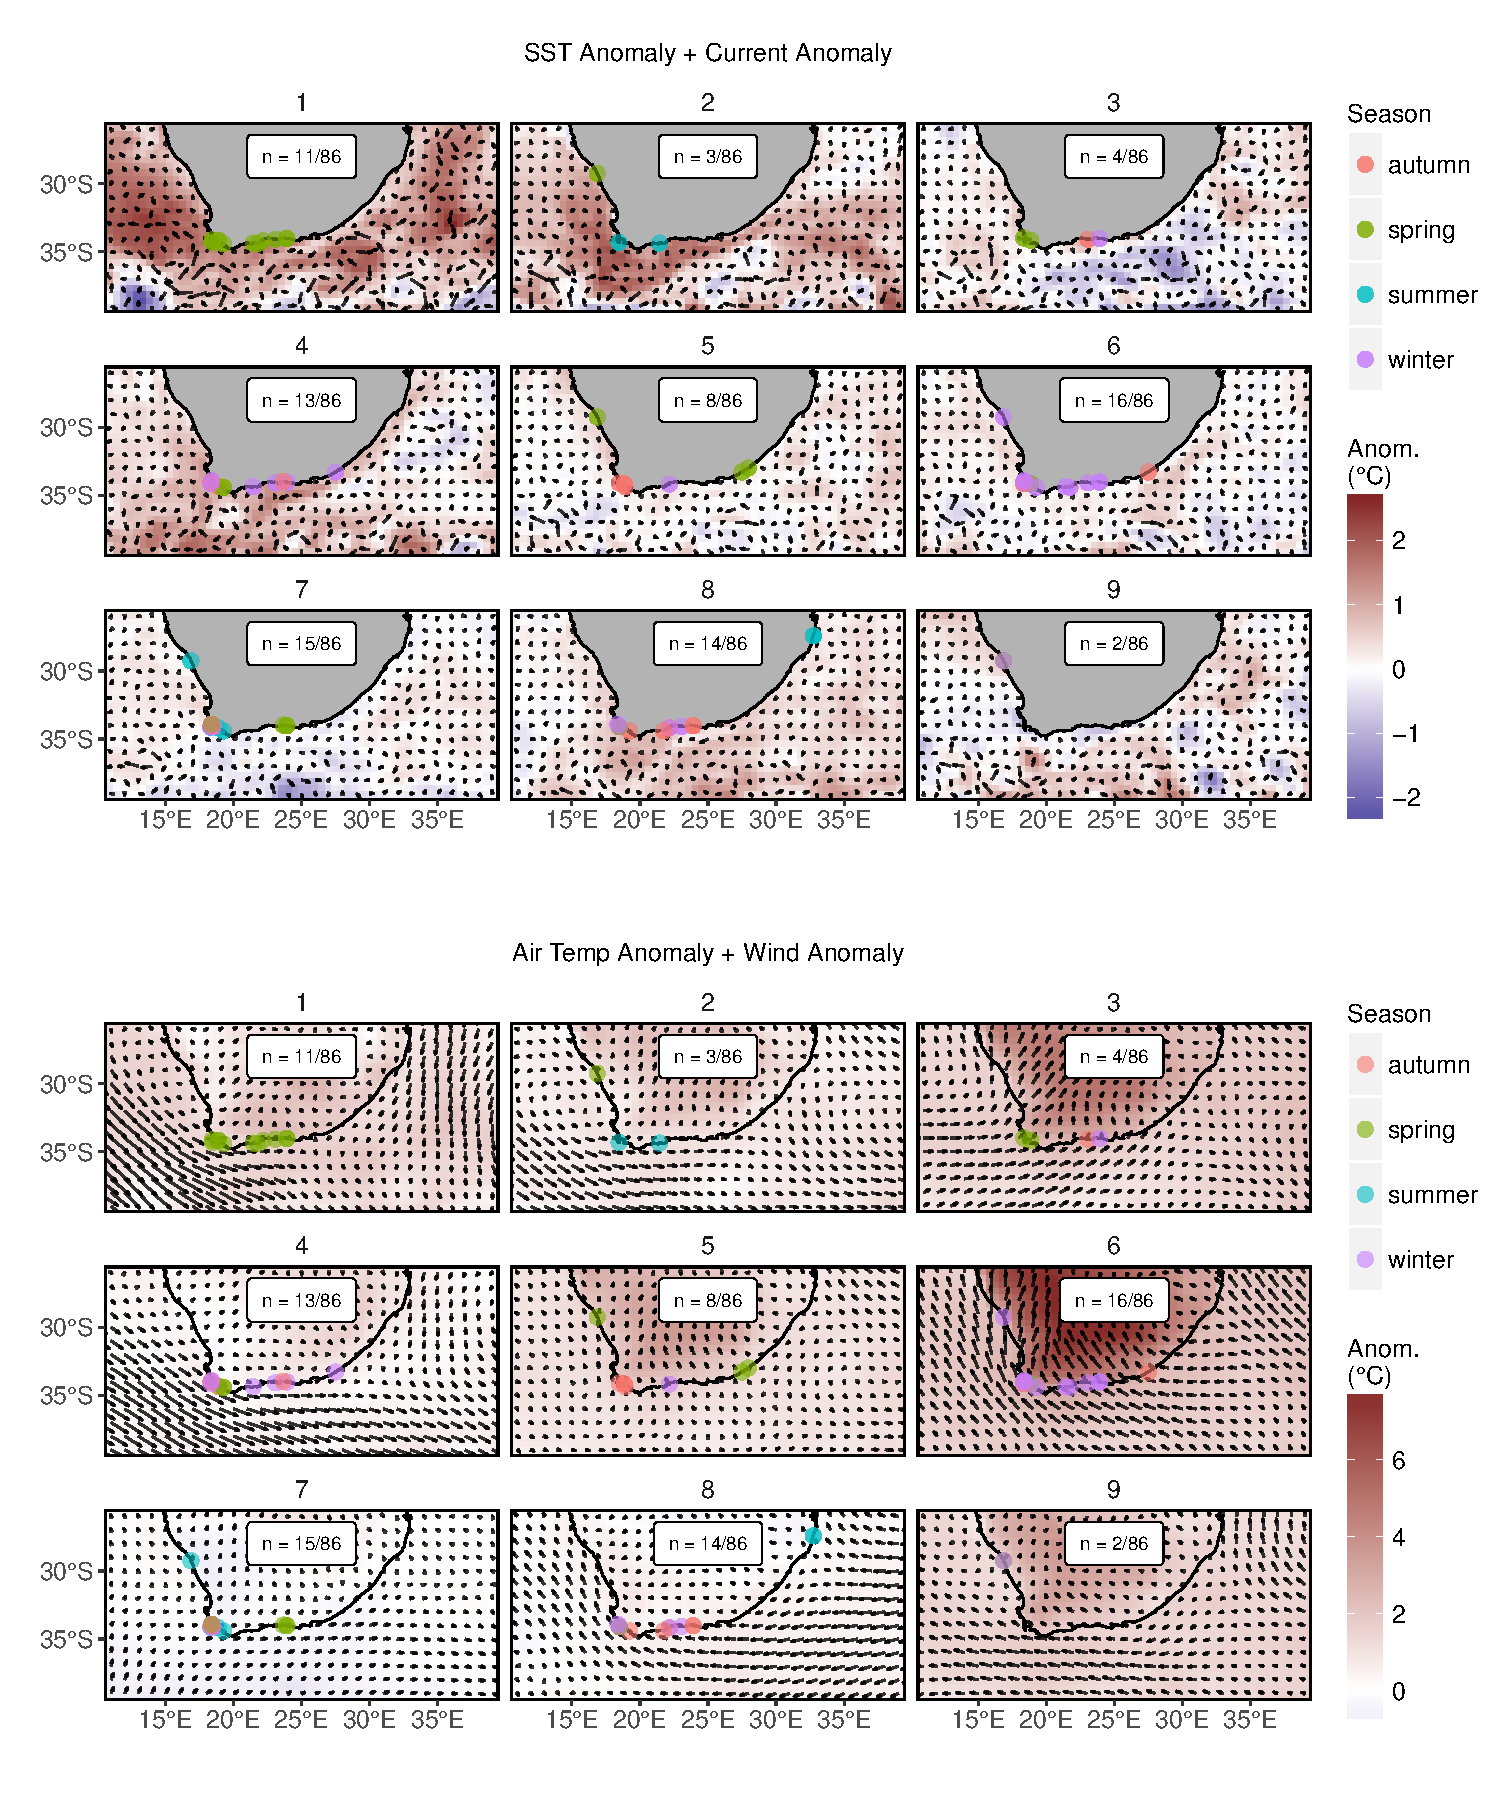
\includegraphics[width=1.0\textwidth]{figure_4.pdf}
\end{center}
\caption{Predominant anomalous atmospheric and oceanic patterns during coastal marine heatwaves (MHWs) as determined by a SOM. The top nine panels show the oceanic patterns while the bottom nine panels show the atmospheric patterns. The current and wind vectors are the same scale as those found in the respective atmospheric and oceanic panels of figure \ref{figure1}. The number of events clustered into each node is shown within the white label in the middle of each panel. The location of each coastal MHW within each node is shown with a dot whose colour denotes the season during which that event occurred/started. Note that the temperature anomaly scales differ for the top and bottom nine panels.}
\label{figure4}
\end{figure}

\begin{figure}[]
\begin{center}
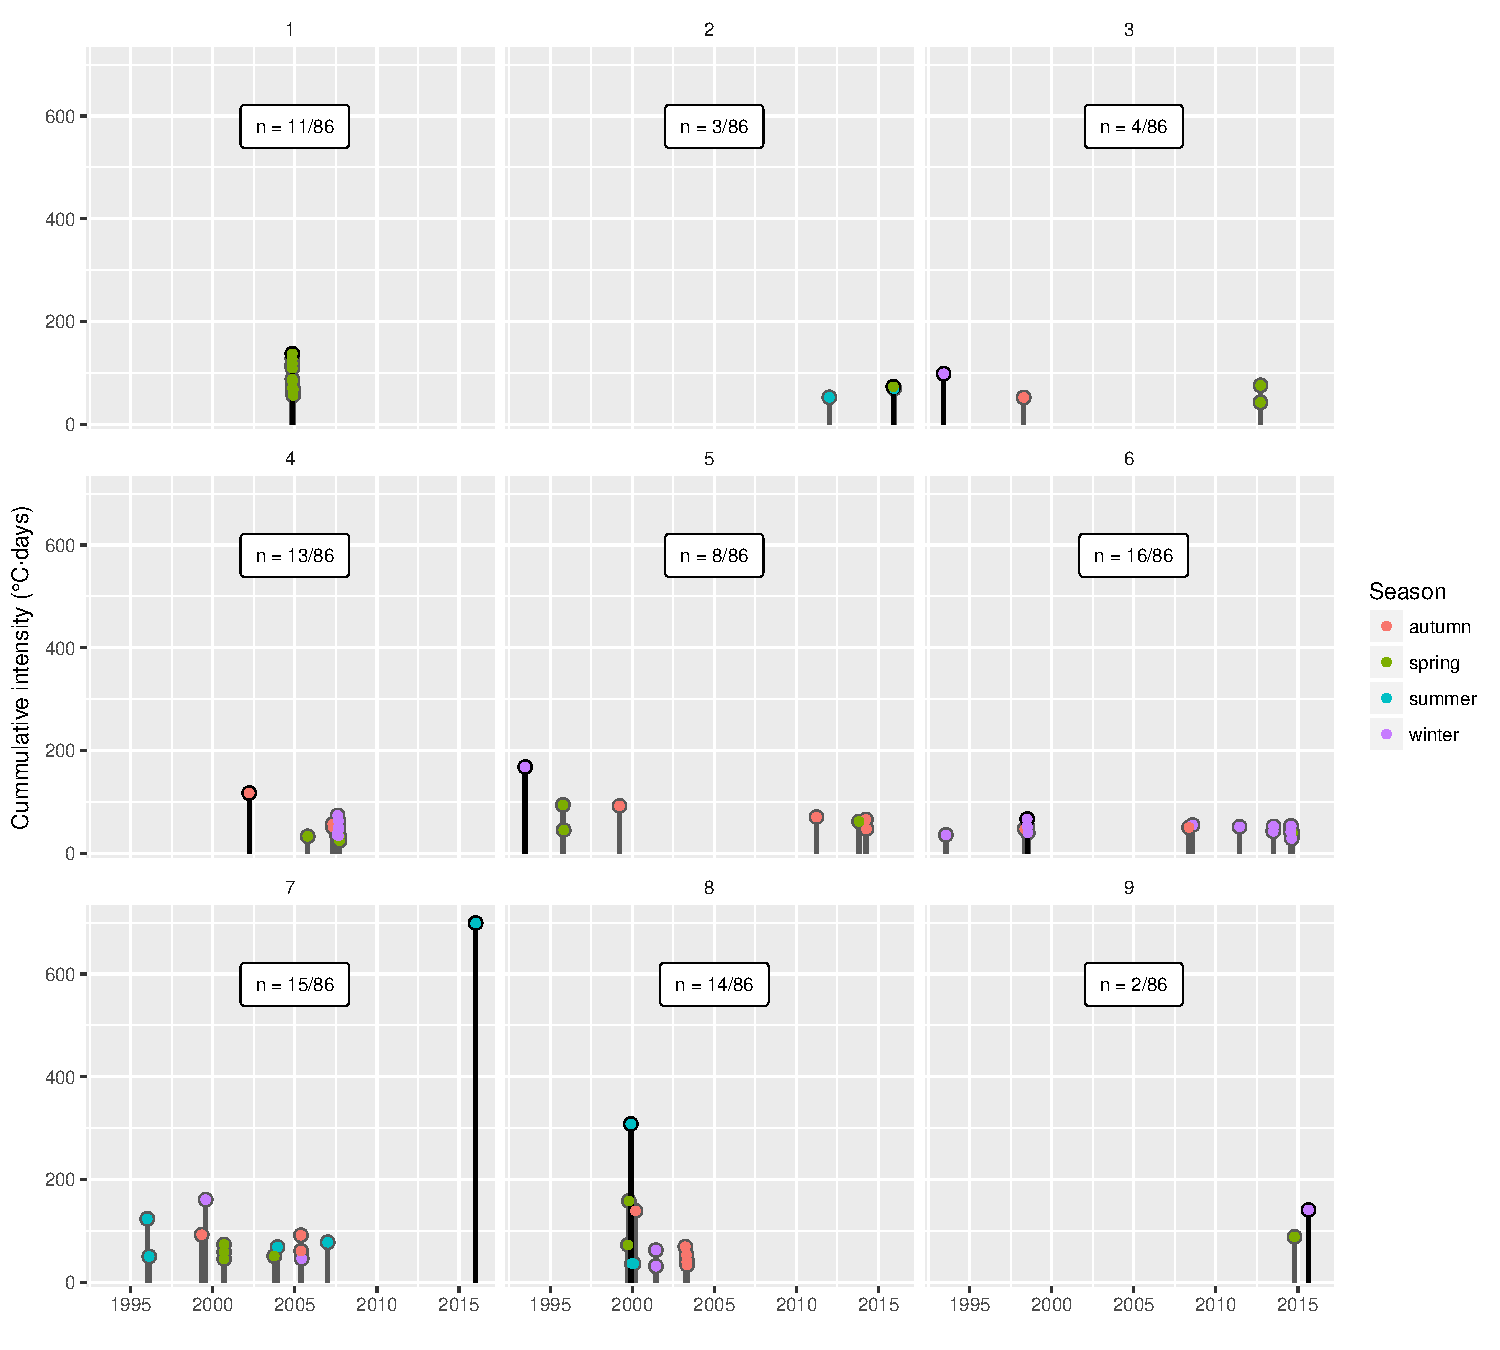
\includegraphics[width=1.0\textwidth]{figure_5.pdf}
\end{center}
\caption{Lolliplot showing the start date for each marine heatwave (MHW) within each node as seen in figure \ref{figure4}, with the number portion of total events per node shown within the white label in the middle of each panel. The height of each lolli shows the cumulative intensity of the event, as outlined in table \ref{table1}, while the lolli colour denotes the season during which the event occurred/started.}
\label{figure5}
\end{figure}


\section*{Table captions}

\begin{table}[ht]
\caption{The descriptions for the metrics of MHWs as proposed by \citet{Hobday2016} and adapted from \citet{Schlegel2017}.}
\label{table1}
\centering
\tiny
\begin{tabular}{ll}
\toprule
 Name [unit] & Definition \\
 \midrule
  Count [no. events per year] & \emph{n}: number of MHWs per year \\
  Duration [days] & \emph{D}: Consecutive period of time that temperature exceeds the threshold \\
  Maximum intensity [\degree C] & \emph{i\textsubscript{max}}: highest temperature anomaly value during the MHW \\
  Mean intensity [\degree C] & \emph{i\textsubscript{mean}}: mean temperature anomaly during the MHW \\
  Cumulative intensity [\degree C$\cdot$days] & \emph{i\textsubscript{cum}}: sum of daily intensity anomalies over the duration of the event \\
  Onset rate [\degree C$/$day] & \emph{r\textsubscript{onset}}: daily increase from event onset to maximum intensity \\
  Decline rate [\degree C$/$day] & \emph{r\textsubscript{decline}}: daily decrease from maximum intensity to event end \\
  \bottomrule
  \end{tabular}
\end{table}

\begin{table}[ht]
\caption{The count of MHWs clustered into each node, count of events for each season, count of events for each coast, and relevant metrics for those MHWs. The mean duration of the events within each node are shown in column \emph{D} with the \emph{i\textsubscript{cum}} and \emph{i\textsubscript{max}} columns showing the mean cumulative and maximum intensities respectively (table \ref{table1}). The bottom row of each column shows the sum or mean of the column as appropriate.}
\label{table2}
\centering
\tiny
\begin{tabular}{cccccccccccc}
  \toprule
Node & Count & Summer & Autumn & Winter & Spring & West & South & East & \emph{D} & \emph{i\textsubscript{cum}} & \emph{i\textsubscript{max}} \\
  \midrule
  1 &  11 &   0 &   0 &   0 &  11 &   0 &  11 &   0 & 33.50 & 93.73 & 4.04 \\
  2 &   3 &   2 &   0 &   0 &   1 &   1 &   2 &   0 & 21.30 & 64.88 & 4.05 \\
  3 &   4 &   0 &   1 &   1 &   2 &   1 &   3 &   0 & 25.80 & 67.19 & 3.49 \\
  4 &  13 &   0 &   3 &   7 &   3 &   4 &   9 &   0 & 25.20 & 51.07 & 2.89 \\
  5 &   8 &   0 &   4 &   1 &   3 &   1 &   6 &   1 & 29.00 & 80.52 & 4.75 \\
  6 &  16 &   0 &   2 &  13 &   1 &   5 &  11 &   0 & 23.40 & 47.59 & 2.94 \\
  7 &  15 &   6 &   3 &   2 &   4 &   8 &   7 &   0 & 41.10 & 118.55 & 4.21 \\
  8 &  14 &   3 &   6 &   3 &   2 &   1 &  11 &   2 & 28.20 & 79.50 & 3.94 \\
  9 &   2 &   0 &   0 &   1 &   1 &   2 &   0 &   0 & 46.00 & 114.56 & 4.78 \\
  ALL &  86 &  11 &  19 &  28 &  28 &  23 &  60 &   3 & 29.90 & 77.72 & 3.73 \\
  \bottomrule
  \end{tabular}
\end{table}

\begin{table}[ht]
\caption{Qualitative descriptions and groupings of the predominant atmospheric or oceanic patterns present across the SOM nodes.}
\label{table3}
\centering
\tiny
\begin{tabular}{llll}
  \toprule
Node & Coast & Season & Pattern \\ 
  \midrule
(1,2,4) & West, South & All & Warm SSTs with onshore forcing, cool air with W/NW-erly wind anomalies \\ 
  (3,5,6,9) & All & All & Cool or neutral offshore SSTs, warm air with mostly onshore wind anomalies \\ 
  (8) & All & All & Warm SSTs with no onshore forcing, neutral air with E/SE-erly wind anomalies \\ 
  (7) & West, South & All & Neutral \\ 
  \bottomrule
  \end{tabular}
\end{table}

\end{document}